\documentclass[tikz, border=50pt]{standalone}

\usepackage{tikz}
\usepackage{medl_colors}
\usepackage{graphicx}
\usetikzlibrary{shapes.multipart, shapes.geometric, arrows.meta}
\usetikzlibrary{matrix, calc, positioning,fit}
\usepackage{xstring}

\begin{document}
\begin{tikzpicture}

%images
\node[scale = .4] (interpolation3_1)  {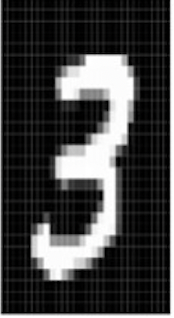
\includegraphics {images/interpolation3_1.png}};
\node[scale = .4, right of=interpolation3_1, node distance=10cm] (interpolation3_3)  {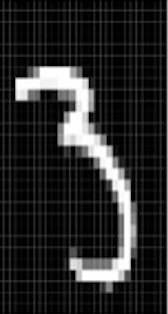
\includegraphics {images/interpolation3_3.png}};
\node[scale = .4, above of = interpolation3_1, node distance = 8cm, xshift=5cm] (interpolation3_2)  {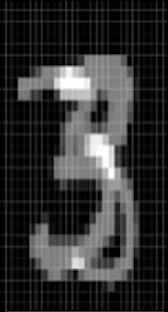
\includegraphics {images/interpolation3_2.png}};
\node[scale = .4, below of = interpolation3_2, node distance = 16cm] (interpolation3_4)  {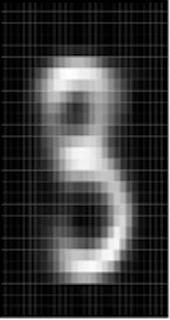
\includegraphics {images/interpolation3_4.png}};

%labels
\node[node distance = 1.5cm, align=center, below of = interpolation3_1] { $x^{(i)}$};
\node[node distance = 1.5cm, align=center, below of = interpolation3_2] { $x_\lambda^\text{naive}$};
\node[node distance = 1.5cm, align=center, below of = interpolation3_3] { $x^{(j)}$};
\node[node distance = 1.5cm, align=center, below of = interpolation3_4] { $x_\lambda^\text{encoder}$};


\end{tikzpicture}
\end{document}